\documentclass[cn]{homework}

\title{第八次作业}

\begin{document}
    \maketitle

    \problem
    % TODO deduction of limit dist of t-statistic

    \problem
    不妨设$Y_0=0$,
    \[Y_t=Y_{t-1}+\varepsilon_t,\quad
    \varepsilon_t\overset{\text{i.i.d.}}\sim\mathcal N(0,\sigma^2)\]
    分别选择$\sigma^2=1,4$,
    模拟如\cref{fig:simulation}。
    \begin{figure}[h]
        \centering
        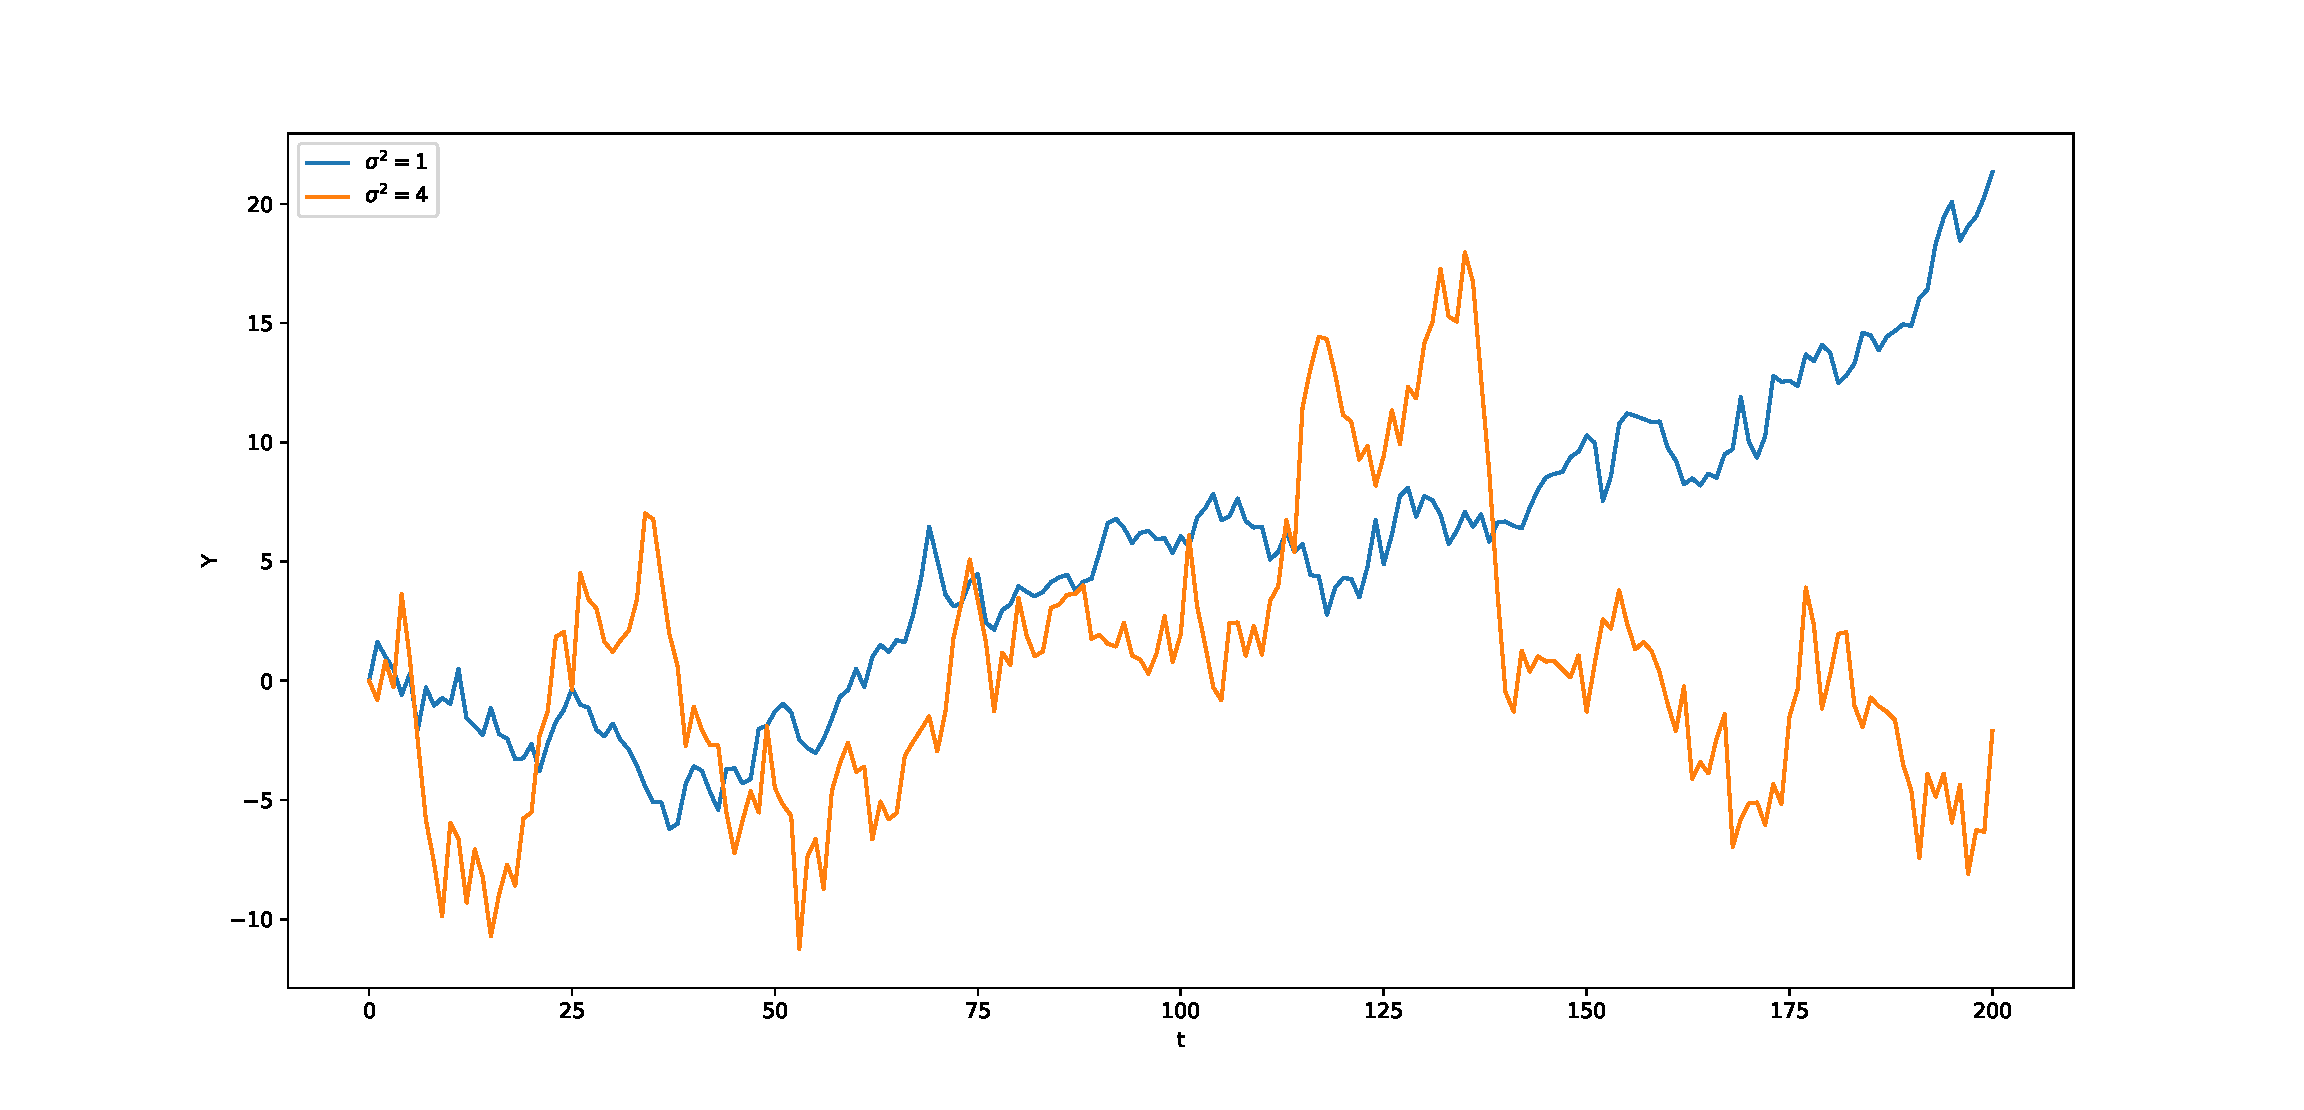
\includegraphics[width=\linewidth]{simulation}
        \caption{随机游走模拟}
        \label{fig:simulation}
    \end{figure}

    \appendix
    \section{随机游走代码(Python)}
    \lstinputlisting[language=Python]{simulation.py}
\end{document}